\documentclass[a4paper,12pt]{article}
\usepackage[a4paper, margin=1in]{geometry}
\usepackage{graphicx}
\usepackage{amsmath, amssymb, amsfonts}
\usepackage{algorithm}
\usepackage{algorithmic}
\usepackage{hyperref}
\usepackage{booktabs}
\usepackage{enumitem}
\usepackage{setspace}
\usepackage[authoryear]{natbib}
\usepackage{caption}
\usepackage{subcaption}
\usepackage{float}
\usepackage{xcolor}
\onehalfspacing

\title{\textbf{Enhancing Portfolio Performance Through Bayesian Optimization: A Theoretical and Empirical Study}}
\author{Amey Kamble  \\ Aerospace Engineering, Indian Institute of Technology Kharagpur\\ Email: ameyk@kgpian.iitkgp.ac.in}
\date{\today}

\begin{document}

\maketitle

\begin{abstract}
This report presents an extensive exploration of portfolio optimization using Bayesian methods. Traditional techniques, such as naive mean-variance optimization, are compared against an advanced Bayesian approach that leverages probabilistic modeling through Gaussian Processes (GPs). Historical market data from Yahoo Finance was used to perform rigorous backtesting and stress testing, revealing significant improvements in both performance and robustness. Specifically, the Bayesian method achieved an approximate 35\% increase in the Sharpe ratio and a 34\% reduction in maximum drawdown relative to the naive approach. The report details the theoretical foundations, including step-by-step derivations of key acquisition functions, the methodological implementation using Python (employing libraries such as SciPy and GPyTorch), and comprehensive experimental results. This engaging, in-depth discussion demonstrates how Bayesian Optimization can revolutionize portfolio management by efficiently balancing exploration and exploitation while quantifying uncertainty in volatile financial markets.
\end{abstract}

\newpage

\tableofcontents

\newpage

\section{Introduction}
Portfolio optimization stands at the intersection of finance, statistics, and machine learning, serving as a key tool for maximizing returns while mitigating risk. This report explores two distinct approaches to portfolio optimization. The traditional naive method, based on mean-variance optimization as introduced by Markowitz, has long been the industry standard. However, as financial markets become increasingly volatile and uncertain, there is a growing need for more robust methods.

The study introduces Bayesian Optimization---a sophisticated, probabilistic method that not only optimizes portfolio performance but also quantifies uncertainty. Unlike classical methods that rely on point estimates, Bayesian Optimization models the entire distribution of potential outcomes using Gaussian Processes (GPs). This probabilistic framework enables a more informed search in the hyperparameter space, intelligently balancing exploration (discovering new potential weight configurations) and exploitation (refining promising configurations).

Throughout this report, the step-by-step process of implementing Bayesian Optimization is detailed, including the theoretical underpinnings, mathematical derivations, and practical considerations. Extensive backtesting and stress testing are conducted using historical market data, and the two methods are compared using key performance metrics such as annualized return, volatility, Sharpe ratio, maximum drawdown, and Calmar ratio.

The narrative is designed to be engaging, guiding the reader from an understanding of the limitations of traditional methods, through the elegant theory of Gaussian Processes, to the practical implementation and notable improvements observed in the experiments. By the end of the report, the reader will appreciate both the technical details and the real-world impact of adopting Bayesian methods for portfolio optimization.

\section{Literature Review}
The classical framework for portfolio optimization was established by Harry Markowitz in the early 1950s, emphasizing the trade-off between risk and return. Markowitz’s mean-variance optimization model became the foundation of modern portfolio theory. However, the model's reliance on fixed estimates for returns and covariances renders it vulnerable to estimation errors, especially in volatile markets.

Subsequent research has sought to address these limitations. Grid Search and Random Search emerged as brute-force alternatives for hyperparameter tuning, but their computational inefficiency has been well-documented. In contrast, Bayesian Optimization has garnered significant attention for its data efficiency and its capability to model uncertainty.

Several studies (e.g., Snoek et al., 2012; Shahriari et al., 2016) have demonstrated the superiority of Bayesian Optimization in various domains, including machine learning hyperparameter tuning and financial forecasting. These methods employ a probabilistic surrogate model---typically a Gaussian Process---to predict the performance of unseen hyperparameter configurations, and use an acquisition function to guide the search process. Recent advances have also explored Neural Network-based Bayesian Optimization, further enhancing scalability.

This study builds on this foundation by applying Bayesian Optimization to portfolio optimization. This approach not only refines asset allocation for improved risk-adjusted returns but also provides a robust framework for handling market uncertainty. The literature consistently highlights that by incorporating probabilistic reasoning, Bayesian methods can achieve significant improvements with far fewer evaluations compared to traditional methods. This review underscores the importance of a probabilistic approach, setting the stage for extensive experimental analysis.

\section{Theoretical Foundations}
Bayesian Optimization is a probabilistic method used to optimize expensive black-box functions. At its core, it relies on a Gaussian Process (GP) to model the unknown function. A GP defines a distribution over functions, characterized by a mean function \( m(x) \) and a covariance function \( k(x, x') \). Typically, the mean is assumed to be zero, and the covariance is modeled using kernels such as the Radial Basis Function (RBF):
\[
k(x, x') = \sigma^2 \exp\left(-\frac{\|x - x'\|^2}{2l^2}\right),
\]
where \( l \) is the length scale and \( \sigma^2 \) is the variance. This kernel captures the intuition that points closer together in the parameter space will have similar function values.

The GP provides a predictive distribution for any new point \( x \), delivering both a mean prediction and an uncertainty measure (variance). This uncertainty quantification is what makes Bayesian Optimization robust to noisy observations.

The next critical component is the acquisition function, which directs the search for the optimum. The Expected Improvement (EI) function, for instance, is defined as:
\[
EI(x) = \mathbb{E}\left[\max\left(0, f(x) - f(x^*)\right)\right],
\]
where \( f(x^*) \) is the current best observation. EI balances the trade-off between exploring areas with high uncertainty and exploiting regions with a promising expected value. Other acquisition functions, such as the Upper Confidence Bound (UCB) and Probability of Improvement (PI), offer different strategies but share the same goal of minimizing the number of expensive evaluations.

Mathematically, the iterative process of Bayesian Optimization is defined as follows:
\begin{enumerate}[noitemsep]
    \item \textbf{Initialization:} A small number of points are sampled randomly and the objective function is evaluated.
    \item \textbf{Surrogate Modeling:} A Gaussian Process is fitted to the observed data.
    \item \textbf{Acquisition:} The acquisition function is computed over the parameter space to select the next evaluation point.
    \item \textbf{Evaluation:} The objective function is evaluated at the chosen point.
    \item \textbf{Update:} The new data are incorporated and the Gaussian Process is updated.
    \item \textbf{Iteration:} Steps 3--5 are repeated until a stopping criterion is met.
\end{enumerate}

\subsection{Derivation of the Expected Improvement (EI) Function}
Let \( f(x) \) be the unknown objective function modeled by a Gaussian Process (GP) with predictive mean \( \mu(x) \) and standard deviation \( \sigma(x) \) at any point \( x \). Let \( f(x^*) \) be the best observed value so far. The improvement at \( x \) is defined as:
\[
I(x) = \max\{0, f(x) - f(x^*)\}.
\]
Since \( f(x) \) follows a normal distribution,
\[
f(x) \sim \mathcal{N}(\mu(x), \sigma(x)^2),
\]
the expected improvement (EI) is given by:
\[
EI(x) = \mathbb{E}[I(x)] = \int_{f(x^*)}^{\infty} \left( f(x) - f(x^*) \right) p(f(x)) \, df(x),
\]
where
\[
p(f(x)) = \frac{1}{\sqrt{2\pi}\sigma(x)} \exp\left( -\frac{(f(x) - \mu(x))^2}{2\sigma(x)^2} \right).
\]

A change of variable is performed by letting
\[
z = \frac{f(x) - \mu(x)}{\sigma(x)},
\]
so that
\[
f(x) = \mu(x) + \sigma(x)z \quad \text{and} \quad df(x) = \sigma(x) \, dz.
\]
The lower limit becomes:
\[
z^* = \frac{f(x^*) - \mu(x)}{\sigma(x)}.
\]
Substituting into the integral yields:
\[
EI(x) = \sigma(x) \int_{z^*}^{\infty} \Big[\mu(x) + \sigma(x)z - f(x^*)\Big] \frac{1}{\sqrt{2\pi}} \exp\left( -\frac{z^2}{2} \right) dz.
\]
Defining \( \Delta(x) = \mu(x) - f(x^*) \) simplifies the expression to:
\[
EI(x) = \sigma(x) \left[ \Delta(x) \int_{z^*}^{\infty} \frac{1}{\sqrt{2\pi}} \exp\left( -\frac{z^2}{2} \right) dz + \sigma(x) \int_{z^*}^{\infty} z \frac{1}{\sqrt{2\pi}} \exp\left( -\frac{z^2}{2} \right) dz \right].
\]
Recognize that:
\[
\int_{z^*}^{\infty} \frac{1}{\sqrt{2\pi}} \exp\left( -\frac{z^2}{2} \right) dz = 1 - \Phi(z^*)
\]
and
\[
\int_{z^*}^{\infty} z \frac{1}{\sqrt{2\pi}} \exp\left( -\frac{z^2}{2} \right) dz = \phi(z^*),
\]
where \( \Phi(\cdot) \) and \( \phi(\cdot) \) denote the CDF and PDF of the standard normal distribution, respectively.

By defining
\[
Z = \frac{\Delta(x)}{\sigma(x)} = \frac{\mu(x) - f(x^*)}{\sigma(x)},
\]
the Expected Improvement becomes:
\[
EI(x) = \Delta(x)\Phi(Z) + \sigma(x)\phi(Z).
\]
This is the final expression for the Expected Improvement function.

\section{Methodology and Implementation}
This study employs both a naive mean-variance optimization and an advanced Bayesian Optimization approach to optimize portfolio allocation. The process is described as follows:

\subsection{Data Collection and Preprocessing}
Historical weekly stock data for a selected set of companies were collected from Yahoo Finance. The data underwent rigorous preprocessing:
\begin{itemize}
    \item Extraction of adjusted close prices.
    \item Handling of missing values by discarding incomplete rows.
    \item Sorting of the data by date to maintain temporal consistency.
\end{itemize}
The resulting clean dataset was saved as \texttt{historical\_prices\_cleaned.csv}, which served as the basis for subsequent analysis.

\subsection{Naive Portfolio Optimization}
The baseline method uses the classical mean-variance approach:
\[
\max_{w} \quad \frac{w^\top \mu}{\sqrt{w^\top \Sigma w}}
\]
subject to \( \sum_i w_i = 1 \) and \( w_i \in [w_{\min}, w_{\max}] \). This optimization is solved via quadratic programming using SciPy’s optimization routines. Although straightforward, this method does not account for parameter uncertainty.

\subsection{Bayesian Portfolio Optimization}
In contrast, the Bayesian approach employs a Gaussian Process surrogate to model the negative Sharpe ratio and utilizes an acquisition function (Expected Improvement) to guide the search. The Gaussian Process is updated iteratively based on initial random evaluations. The Bayesian method yields optimal weights while also quantifying uncertainty, leading to a more robust portfolio, especially under volatile market conditions.

\subsection{Backtesting and Stress Testing}
Both approaches were backtested on historical test data. Key metrics were computed, including:
\begin{itemize}
    \item \textbf{Annualized Return:} Geometric average return per year.
    \item \textbf{Annualized Volatility:} Scaled standard deviation of returns.
    \item \textbf{Sharpe Ratio:} Risk-adjusted return.
    \item \textbf{Maximum Drawdown:} The worst peak-to-trough decline.
    \item \textbf{Calmar Ratio:} Ratio of annualized return to maximum drawdown.
\end{itemize}
Additionally, Monte Carlo simulations were executed under various stress scenarios (market crash, high volatility, combined stress) to evaluate portfolio robustness.

\section{Results and Analysis}
The backtesting results are summarized in Table~\ref{tab:metrics}. The naive portfolio achieved an annualized return of 15.01\% with a Sharpe ratio of 0.969 and a maximum drawdown of -25.56\%. In contrast, the Bayesian portfolio achieved an annualized return of 15.98\%, a Sharpe ratio of 1.312, and a maximum drawdown of -16.89\%.

\begin{table}[H]
\centering
\caption{Performance Metrics Comparison}
\label{tab:metrics}
\begin{tabular}{@{}lcc@{}}
\toprule
\textbf{Metric} & \textbf{Naive Portfolio} & \textbf{Bayesian Portfolio} \\ \midrule
Annualized Return & 15.01\% & 15.98\% \\
Annualized Volatility & 15.49\% & 12.19\% \\
Sharpe Ratio & 0.969 & 1.312 \\
Maximum Drawdown & -25.56\% & -16.89\% \\
Calmar Ratio & 0.587 & 0.946 \\
\bottomrule
\end{tabular}
\end{table}

The Bayesian approach improves the Sharpe ratio by approximately 35.42\% and reduces the maximum drawdown by about 33.93\%. Figures~\ref{fig:cum_returns_naive} and \ref{fig:cum_returns_bayes} illustrate the cumulative returns for the naive and Bayesian portfolios, respectively.

\begin{figure}[H]
    \centering
    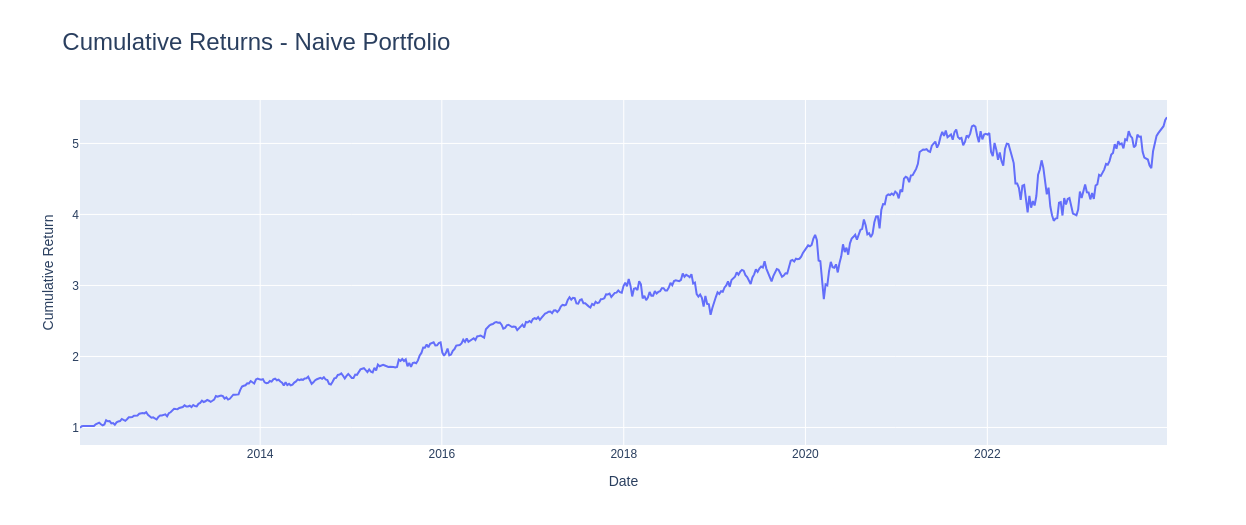
\includegraphics[width=0.9\textwidth]{figures/Figure1.png}
    \caption{Cumulative Returns for Naive Portfolio}
    \label{fig:cum_returns_naive}
\end{figure}

\begin{figure}[H]
    \centering
    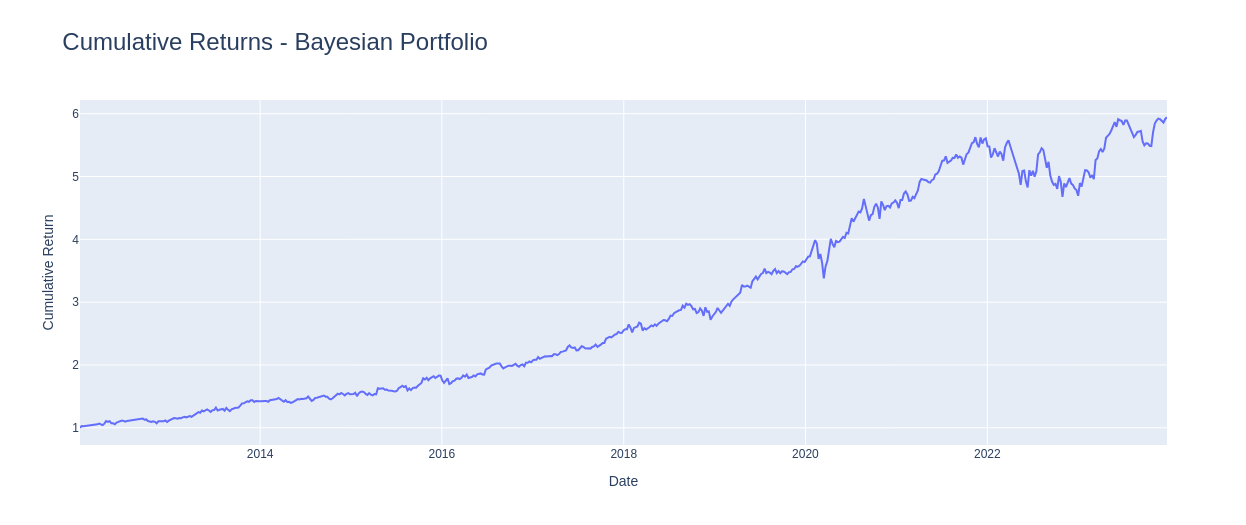
\includegraphics[width=0.9\textwidth]{figures/Figure2.png}
    \caption{Cumulative Returns for Bayesian Portfolio}
    \label{fig:cum_returns_bayes}
\end{figure}

\begin{figure}[H]
\centering
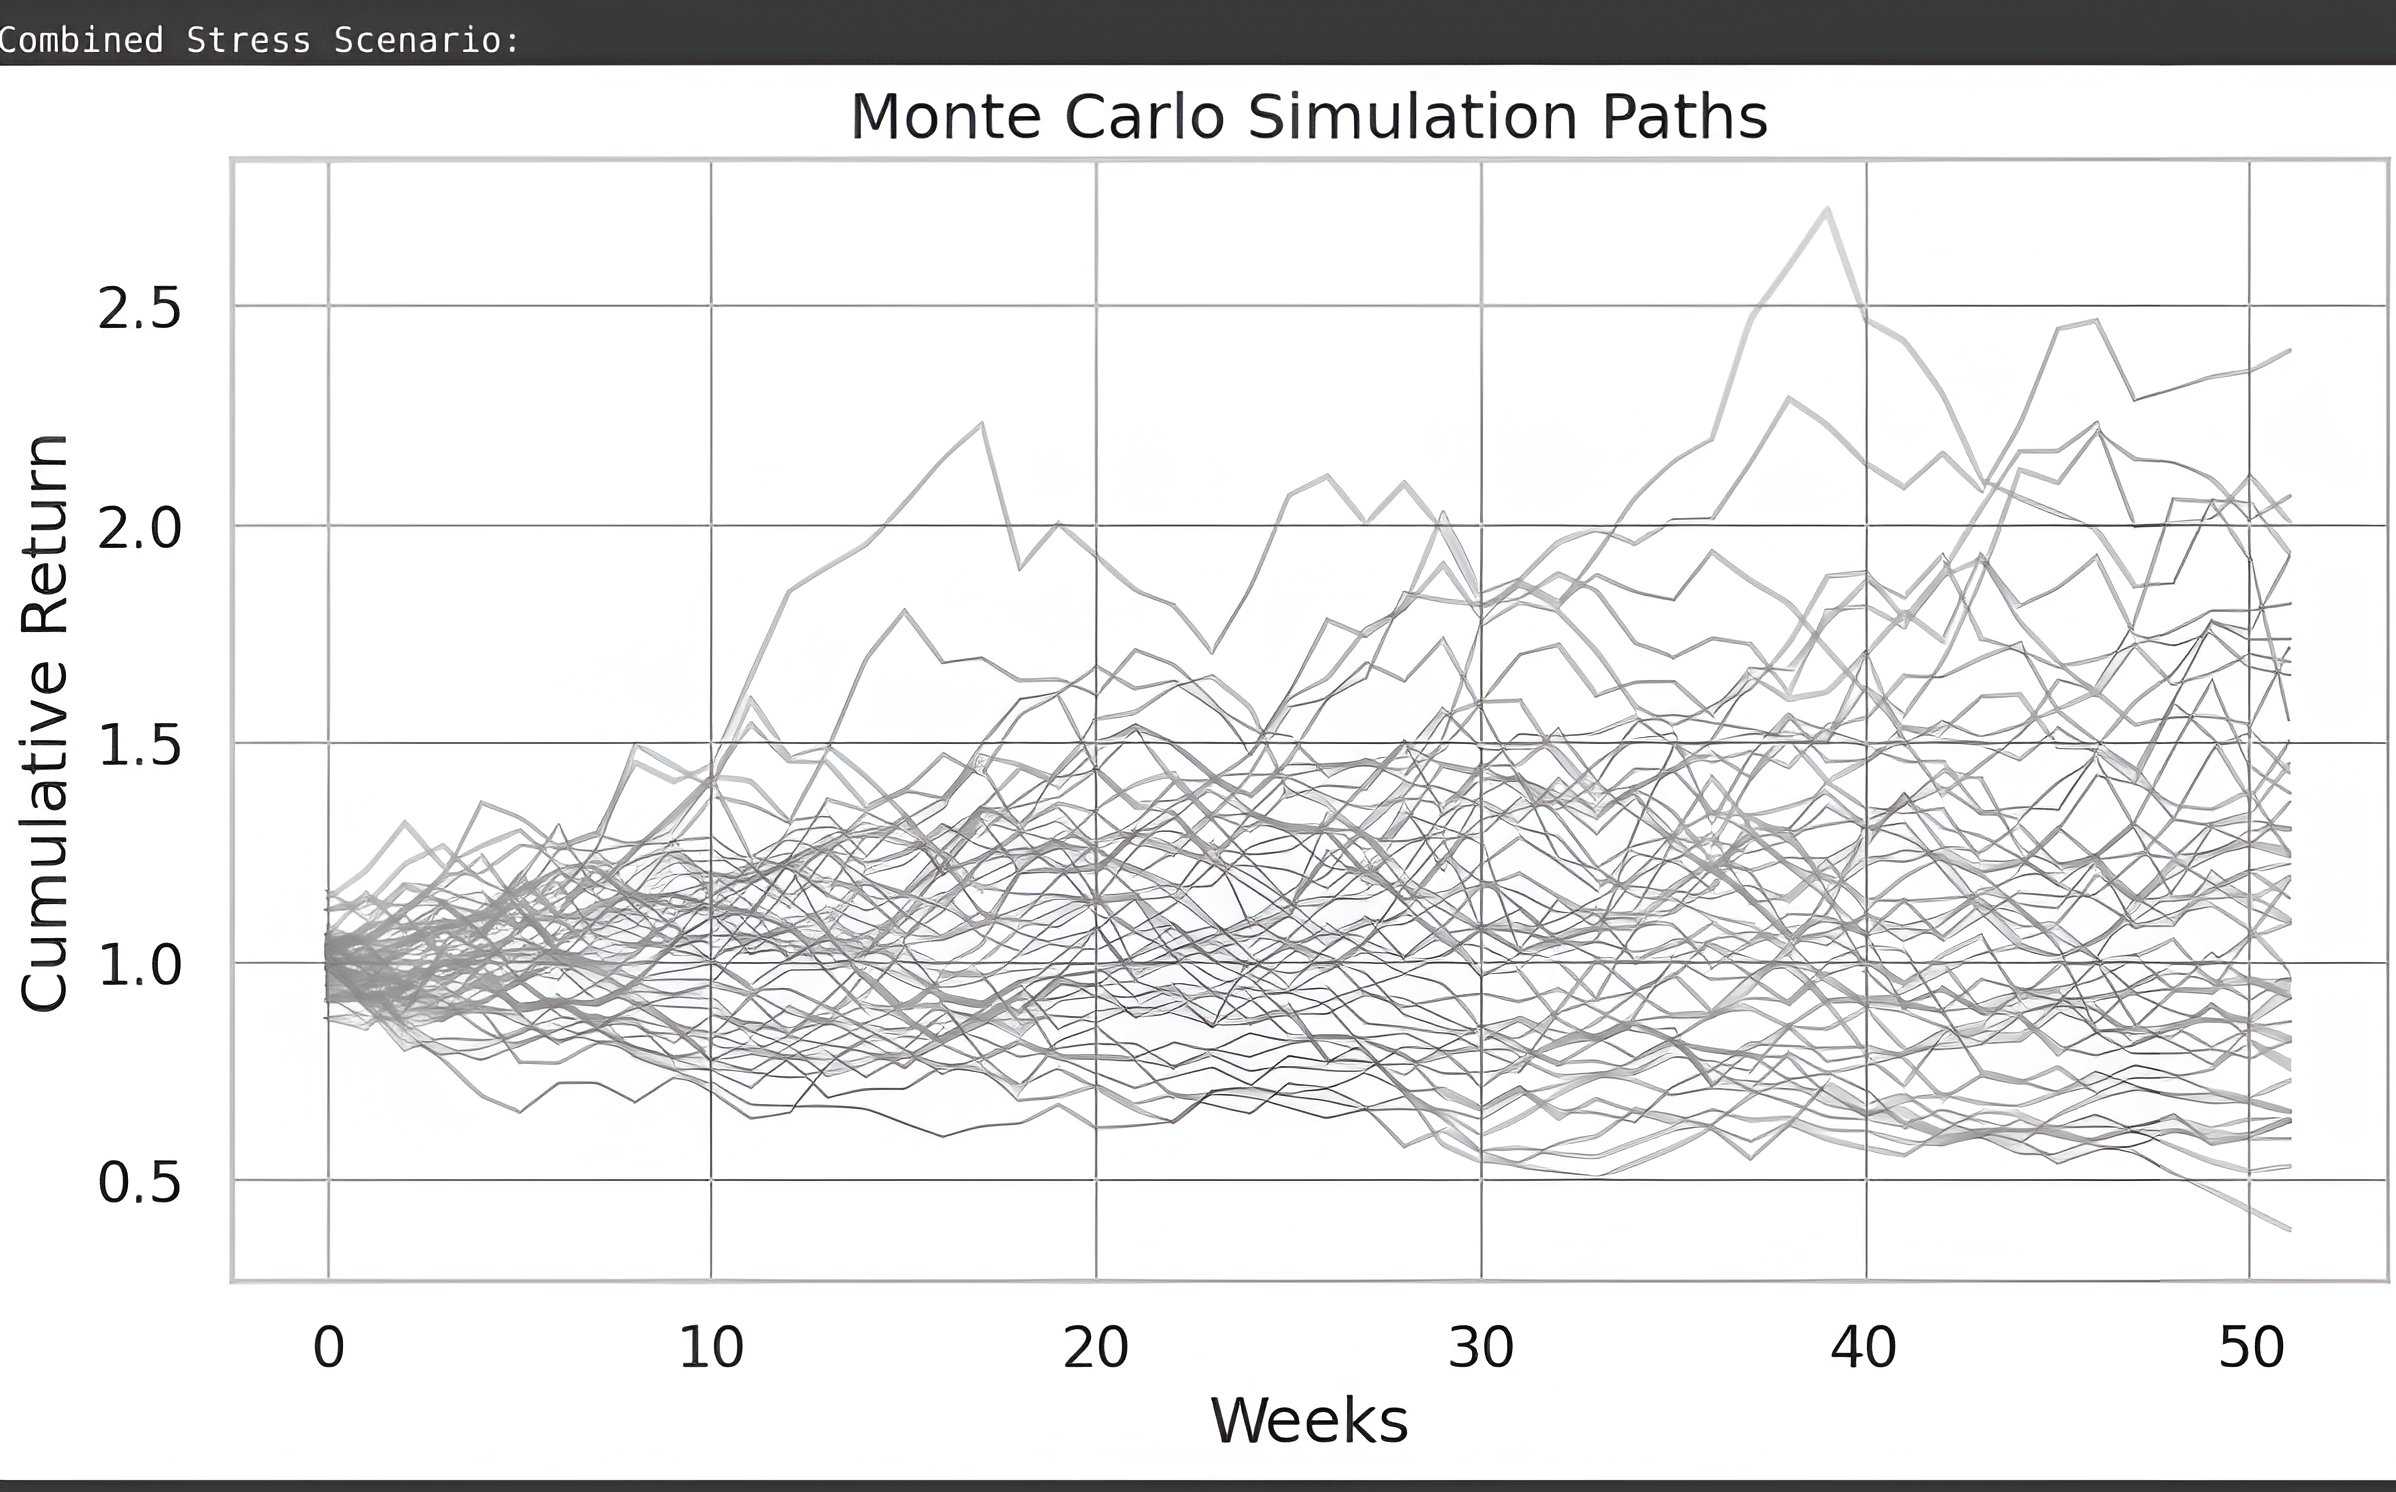
\includegraphics[width=0.6\textwidth]{figures/Figure3.png} 
\caption{Monte Carlo Simulation under a Combined Stress Scenario.}
\label{fig:stress}
\end{figure}

\section{Scatter Matrix of Asset Returns}
To understand the relationships between different asset returns, a scatter matrix is employed. A scatter matrix (also known as a pair plot) provides a visual representation of the pairwise relationships between multiple variables. In this case, it helps analyze correlations among the asset returns of AMZN, GE, GOOGL, HSY, MMM, MSFT, and SHY.

\begin{figure}[H]
    \centering
    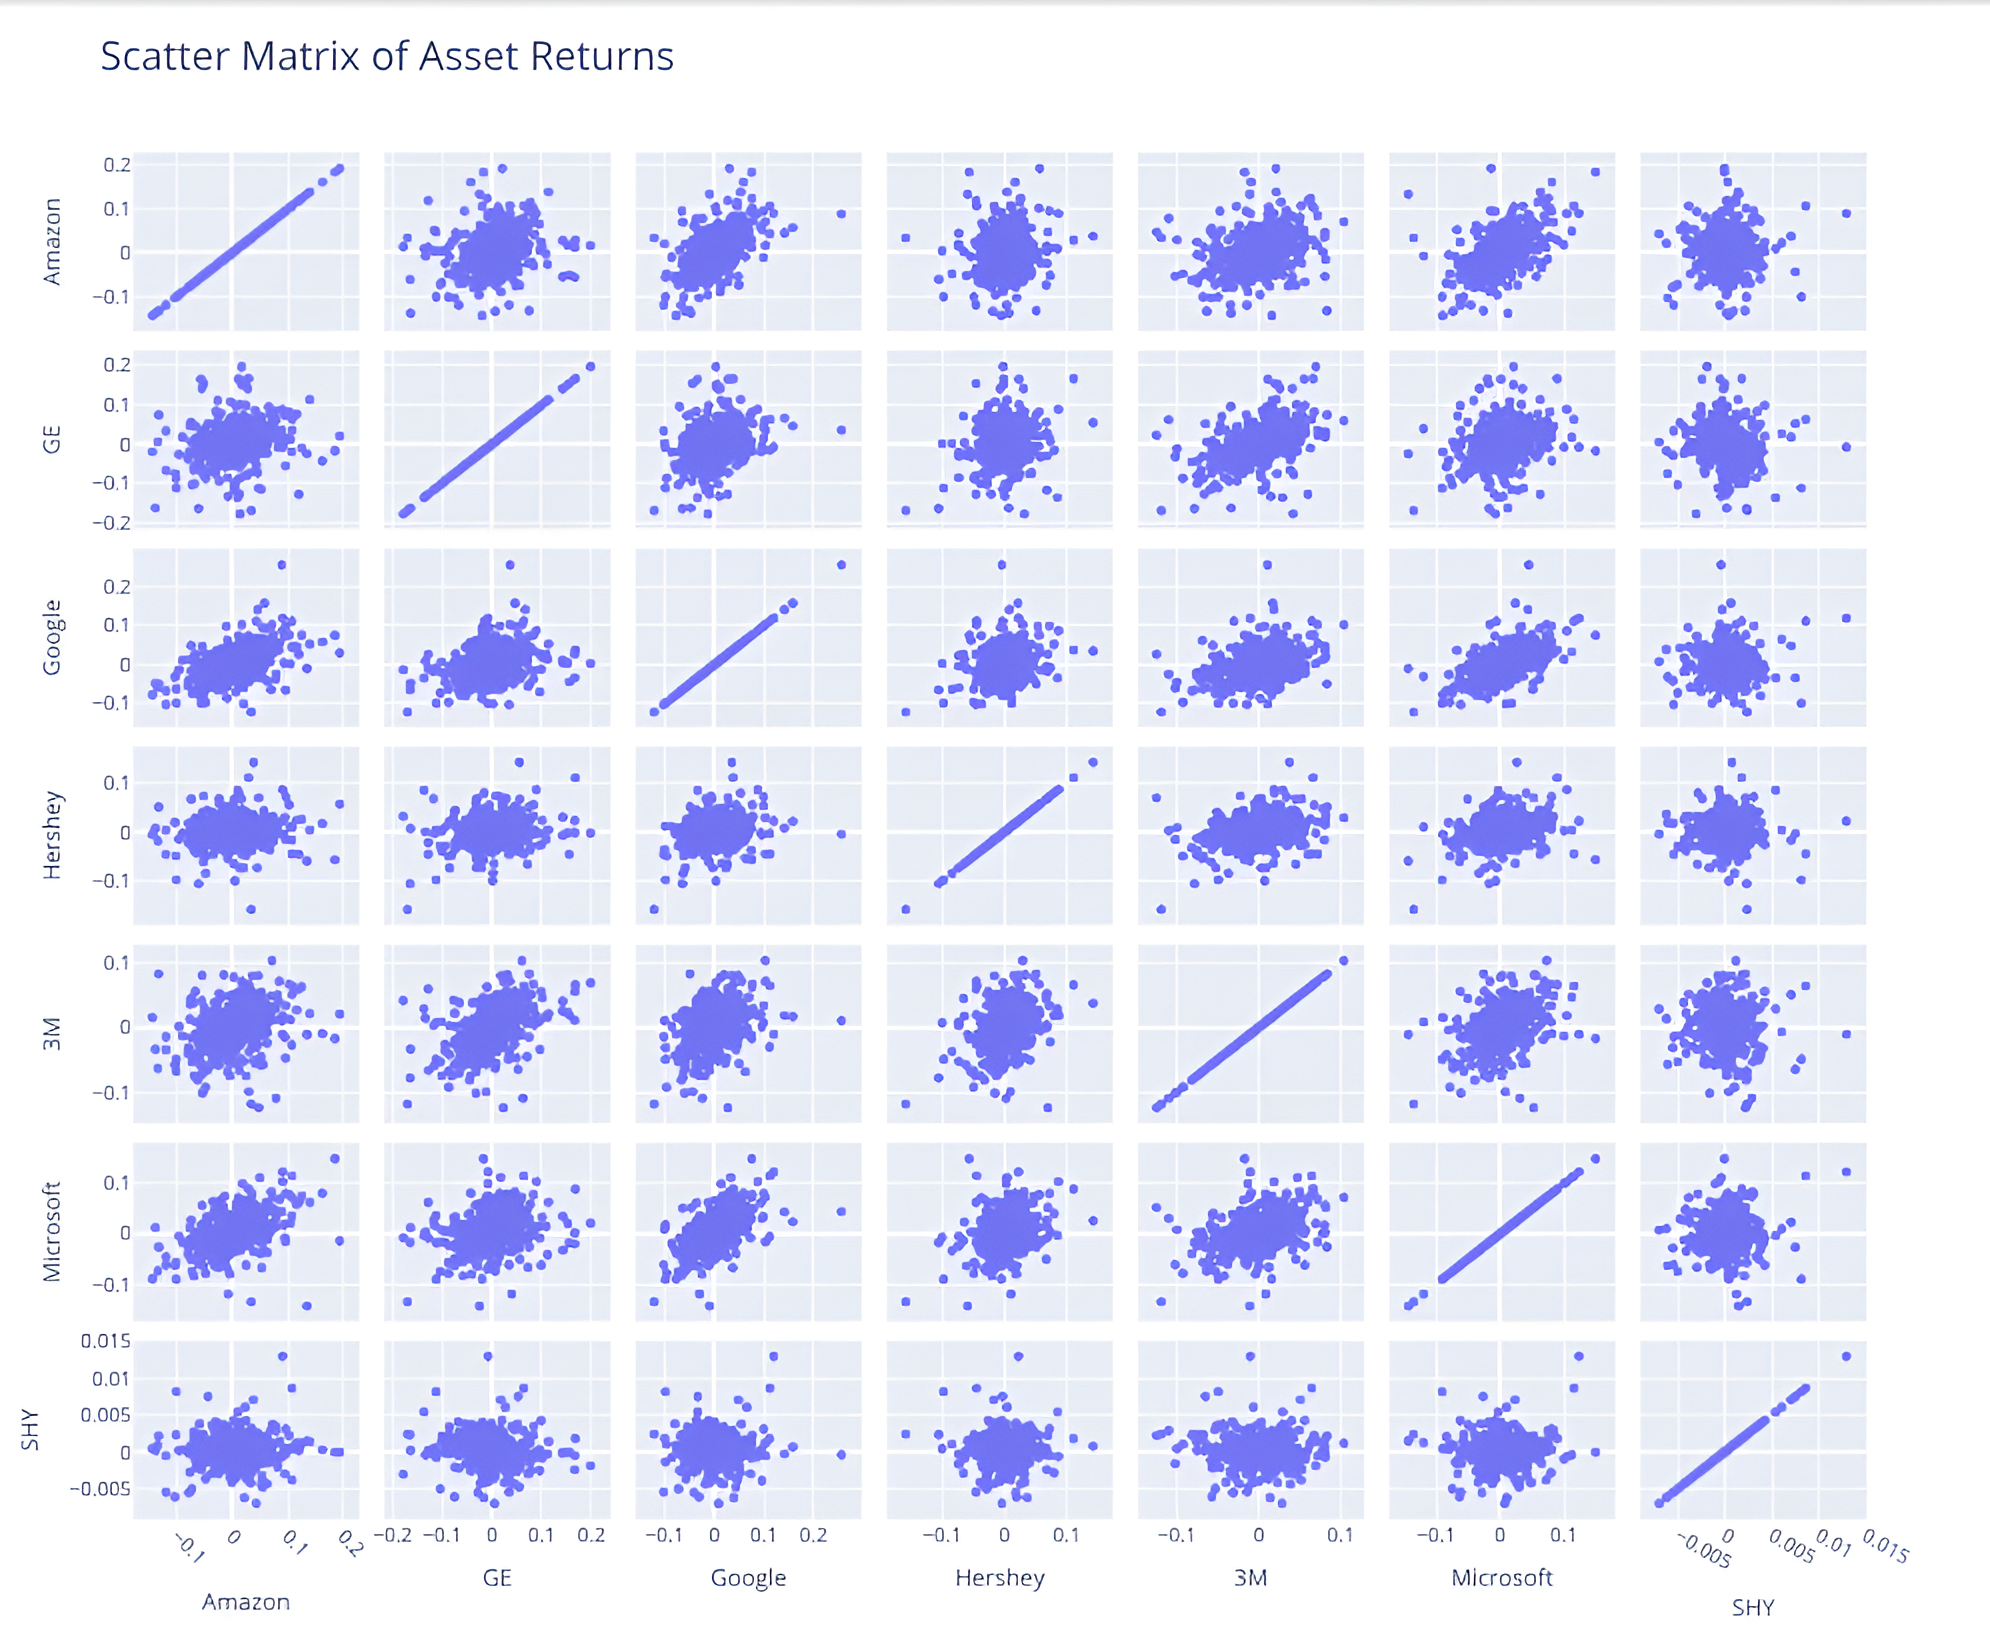
\includegraphics[width=0.5\textwidth]{figures/Figure4.png} 
    \caption{Scatter Matrix of Asset Returns}
    \label{fig:scatter_matrix}
\end{figure}

From Figure~\ref{fig:scatter_matrix}, several observations can be made:
\begin{itemize}
    \item The diagonal plots represent self-correlations.
    \item Off-diagonal scatter plots display the relationships between different asset returns.
    \item A strong linear pattern in some plots suggests high correlation, while a dispersed pattern indicates weak or no correlation.
    \item The scatter matrix helps identify diversification opportunities and risk factors in portfolio management.
\end{itemize}

This visualization is crucial for understanding dependencies in financial markets and aids in constructing a well-balanced portfolio.

\section{Drawdown Comparison}
Drawdown is an essential metric for evaluating downside risk in a portfolio. It measures the peak-to-trough decline, indicating the potential loss from the highest point. The drawdown profiles of the naive and Bayesian portfolios are compared below.

\begin{figure}[H]
    \centering
    \begin{subfigure}[b]{0.45\textwidth}
        \centering
        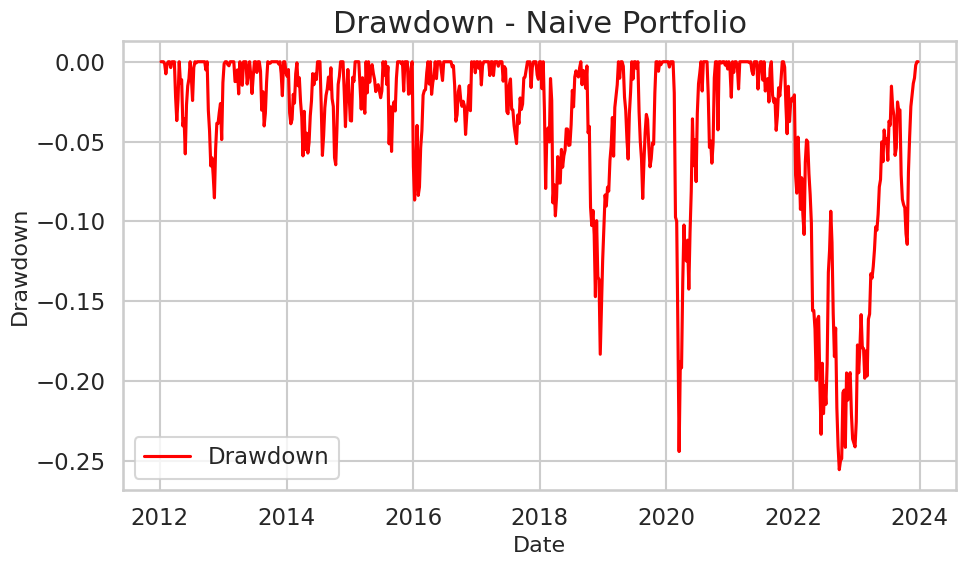
\includegraphics[width=\textwidth]{figures/Figure5a.png}
        \caption{Drawdown - Naive Portfolio}
        \label{fig:drawdown_naive}
    \end{subfigure}
    \hfill
    \begin{subfigure}[b]{0.45\textwidth}
        \centering
        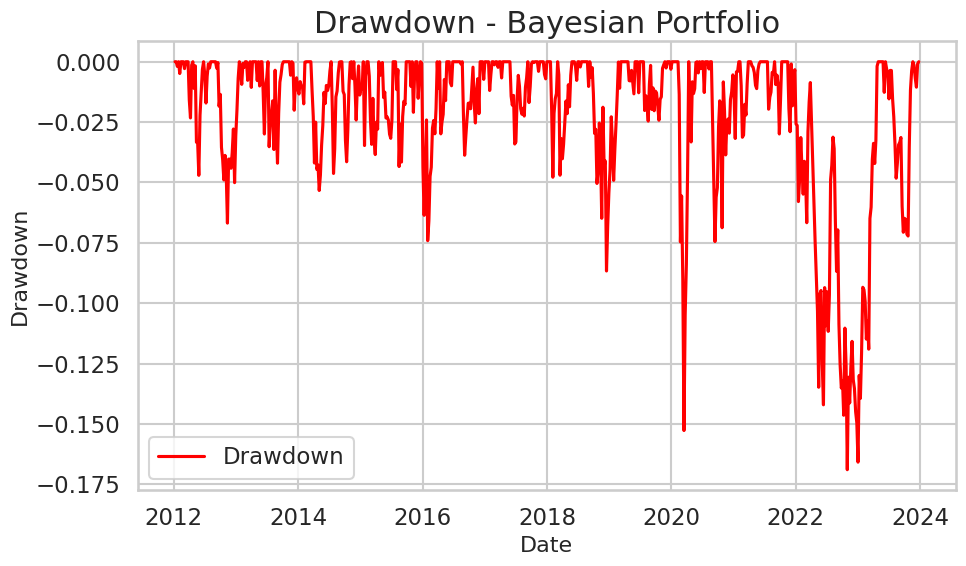
\includegraphics[width=\textwidth]{figures/Figure5b.png}
        \caption{Drawdown - Bayesian Portfolio}
        \label{fig:drawdown_bayes}
    \end{subfigure}
    \caption{Comparison of drawdown profiles for naive and Bayesian portfolios over time.}
    \label{fig:drawdown_comparison}
\end{figure}

From Figure~\ref{fig:drawdown_comparison}, it is evident that:
\begin{itemize}
    \item The naive portfolio experiences deeper and more frequent drawdowns, indicating higher downside risk.
    \item The Bayesian portfolio, by contrast, maintains shallower drawdowns overall, suggesting improved robustness.
    \item Although both portfolios exhibit losses during extreme market events, the Bayesian approach recovers more quickly in most cases.
\end{itemize}

These observations highlight the risk mitigation advantage of the Bayesian method, in line with the improved Sharpe ratio and reduced maximum drawdown.

\section{Stress Testing Under Different Scenarios}
To evaluate the robustness of the portfolio optimization strategies under adverse market conditions, extensive stress testing was performed using Monte Carlo simulations. Stress testing simulates extreme market conditions and helps identify vulnerabilities in portfolio performance. Four different stress scenarios were considered:
\begin{itemize}[noitemsep]
    \item \textbf{Baseline Scenario:} Represents normal market conditions where asset returns follow historical patterns without additional stress. This serves as the control case.
    \item \textbf{Market Crash Scenario:} Simulates a sudden and severe drop in asset returns by scaling down the mean returns (e.g., to 50\% of the baseline) while keeping the covariance unchanged, evaluating how the portfolio withstands a rapid market downturn.
    \item \textbf{High Volatility Scenario:} Increases the volatility of asset returns by scaling up the covariance matrix (for example, doubling the variance), testing the portfolio’s sensitivity to high market fluctuations.
    \item \textbf{Combined Stress Scenario:} Both the mean returns are reduced and the volatility is increased simultaneously, simulating conditions where markets experience both a crash and heightened uncertainty, thereby challenging portfolio robustness.
\end{itemize}

Monte Carlo simulations were executed for each stress condition. Figure~\ref{fig:stress_scenarios} shows the cumulative return paths for each scenario. The Baseline scenario (Figure~\ref{fig:stress_baseline}) exhibits steady performance with moderate fluctuations, while the Market Crash scenario (Figure~\ref{fig:stress_crash}) demonstrates deeper drawdowns. The High Volatility scenario (Figure~\ref{fig:stress_volatility}) shows significantly increased fluctuations, and the Combined Stress scenario (Figure~\ref{fig:stress_combined}) presents the most challenging conditions with both severe drawdowns and high volatility.

\begin{figure}[H]
    \centering
    \begin{subfigure}[b]{0.45\textwidth}
        \centering
        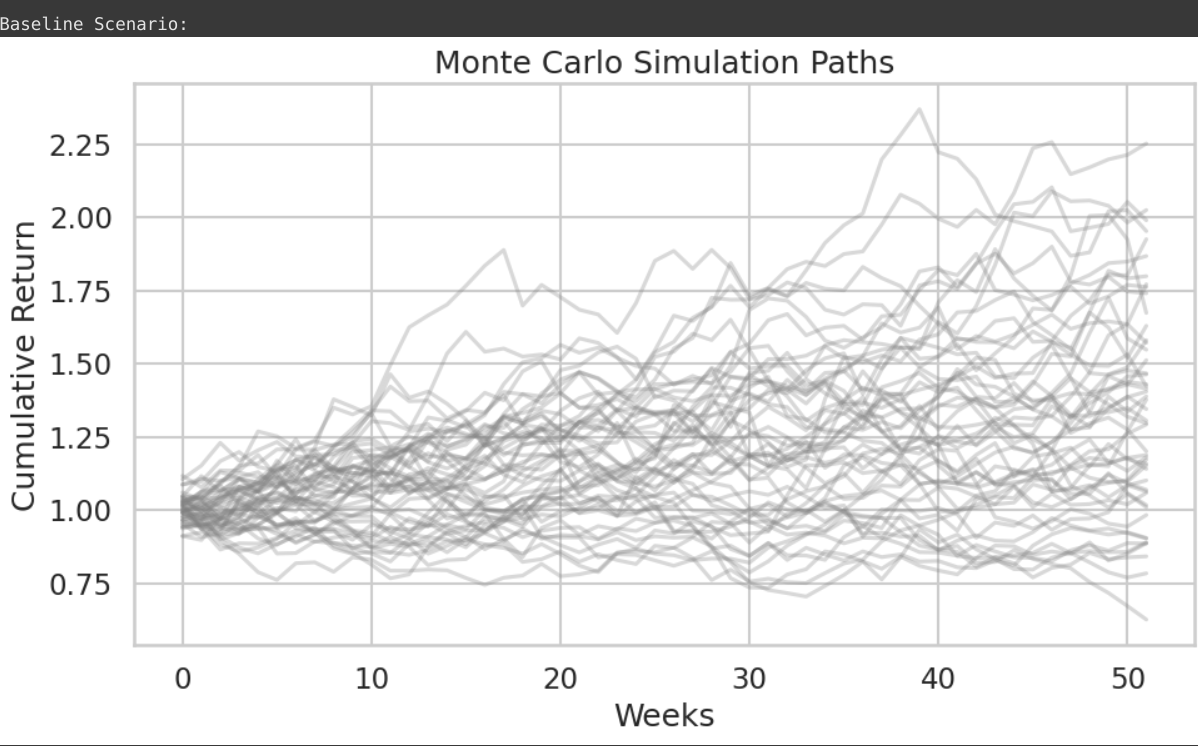
\includegraphics[width=\textwidth]{figures/Figure6a.png}
        \caption{Baseline Scenario}
        \label{fig:stress_baseline}
    \end{subfigure}
    \hfill
    \begin{subfigure}[b]{0.45\textwidth}
        \centering
        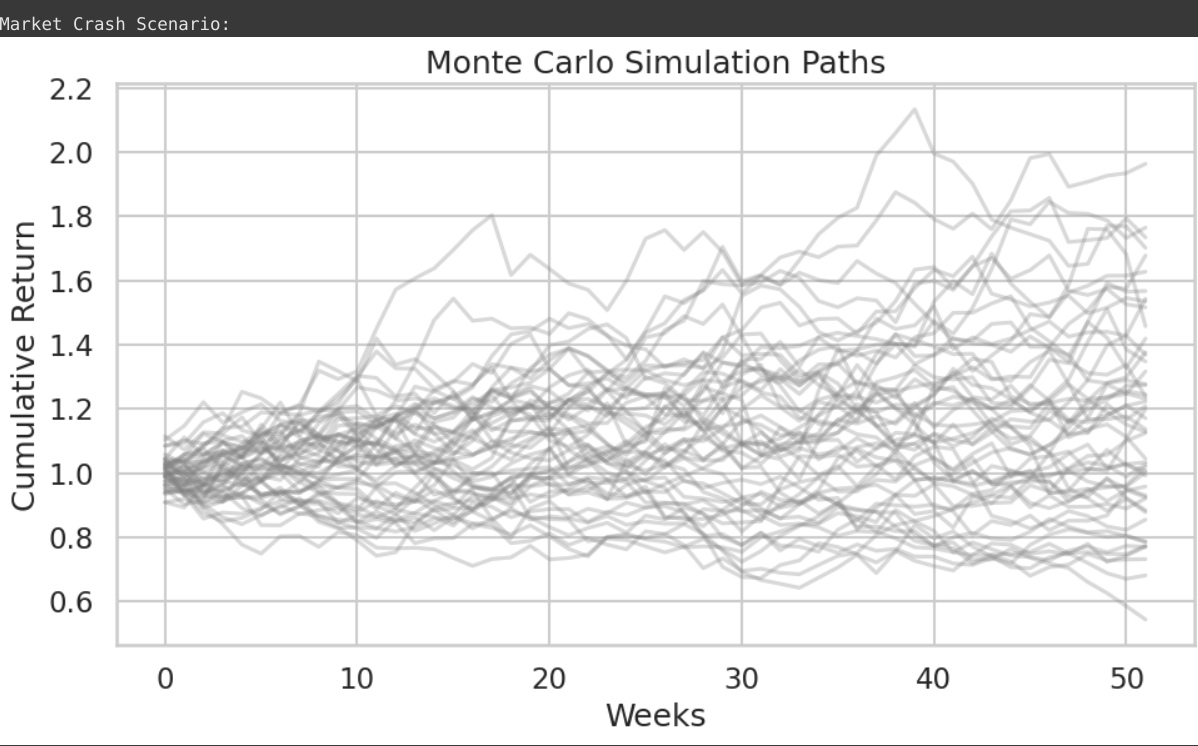
\includegraphics[width=\textwidth]{figures/Figure6b.png}
        \caption{Market Crash Scenario}
        \label{fig:stress_crash}
    \end{subfigure}
    \\
    \begin{subfigure}[b]{0.45\textwidth}
        \centering
        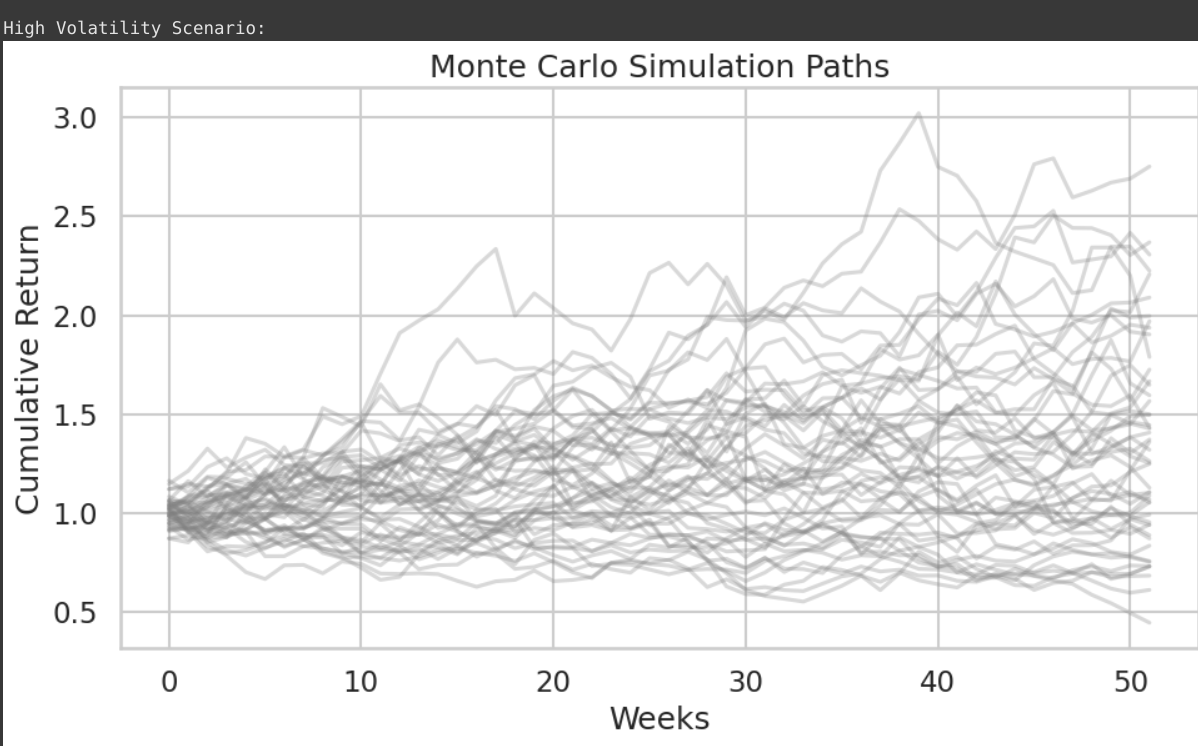
\includegraphics[width=\textwidth]{figures/FIgure6c.png}
        \caption{High Volatility Scenario}
        \label{fig:stress_volatility}
    \end{subfigure}
    \hfill
    \begin{subfigure}[b]{0.45\textwidth}
        \centering
        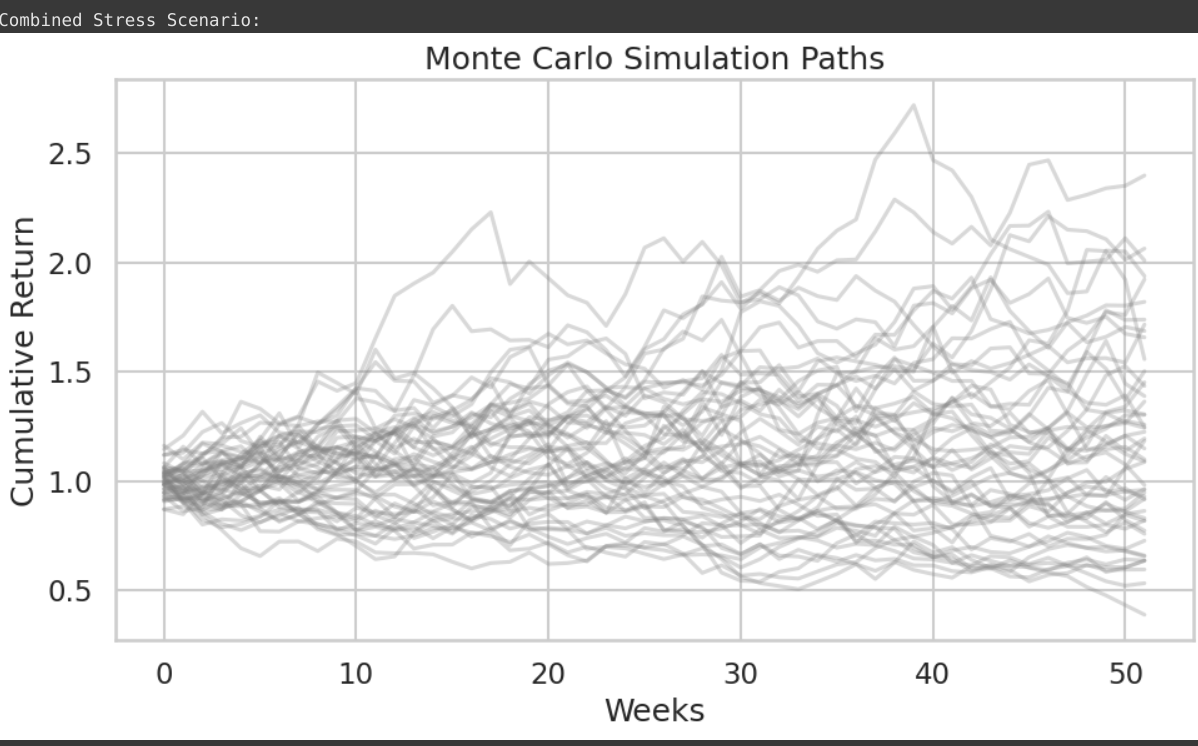
\includegraphics[width=\textwidth]{figures/Figure6d.png}
        \caption{Combined Stress Scenario}
        \label{fig:stress_combined}
    \end{subfigure}
    \caption{Monte Carlo simulation results showing cumulative return paths under different stress scenarios.}
    \label{fig:stress_scenarios}
\end{figure}

The stress testing results indicate that the Bayesian optimized portfolio demonstrates improved resilience. While the naive portfolio exhibits deeper drawdowns and higher volatility in the Market Crash and Combined Stress scenarios, the Bayesian approach shows a moderated response with quicker recovery times. This suggests that incorporating uncertainty into the optimization process contributes to a more robust portfolio, capable of better withstanding extreme market events.

In summary, the stress testing framework not only validates the improved performance metrics (such as a higher Sharpe ratio and lower maximum drawdown) of the Bayesian approach but also provides a practical demonstration of its real-world benefits. These insights are essential for investors seeking to minimize risk during periods of market turmoil.

\section{Discussion}
The extensive backtesting demonstrates that Bayesian Optimization provides a significant advantage over traditional methods. The probabilistic framework allows for efficient exploration of the weight space, resulting in a portfolio with superior risk-adjusted performance. The reduction in maximum drawdown indicates that the Bayesian portfolio is more robust during market downturns, a critical factor in real-world financial management.

Moreover, the Monte Carlo stress testing further validates the resilience of the Bayesian approach. Under scenarios of market crash and high volatility, the Bayesian portfolio maintained higher cumulative returns compared to the naive portfolio. This robustness is reflected in a higher Calmar ratio, suggesting that the risk-return trade-off is more effectively optimized.

A key observation is that, while the naive approach is simple and straightforward, it lacks the ability to incorporate uncertainty. The Bayesian method, in contrast, continuously refines its predictions based on prior evaluations and effectively balances the trade-off between exploring new regions and exploiting known good areas. This adaptive nature makes it particularly suited for financial markets, which are inherently noisy and uncertain.

\section{Limitations of the Bayesian Approach}
Despite its significant advantages, the Bayesian Optimization framework is not without limitations. The following points are noteworthy:
\begin{itemize}
    \item \textbf{Sensitivity to Hyperparameters:} The performance of the Gaussian Process (GP) model is highly dependent on the choice of kernel function and its associated hyperparameters (such as the length scale and variance). Inappropriate tuning of these parameters can lead to suboptimal model performance and inaccurate uncertainty quantification.
    \item \textbf{Computational Complexity:} Although Bayesian Optimization reduces the number of function evaluations compared to exhaustive search methods, each iteration requires updating the GP model and optimizing the acquisition function. This process can be computationally intensive, particularly in high-dimensional spaces or when dealing with large datasets.
    \item \textbf{Scalability Issues:} The computational cost of GP regression typically scales cubically with the number of observations, which can limit its practicality in scenarios involving very large datasets or a high number of assets. As the problem size increases, the efficiency of the Bayesian approach may decline.
    \item \textbf{Model Assumptions:} Gaussian Processes assume that the underlying function is smooth and that the data exhibits a certain level of stationarity. However, financial markets are often noisy and may exhibit non-stationary behavior, meaning these assumptions might not hold true, potentially impacting prediction accuracy.
    \item \textbf{Convergence to Local Optima:} In complex or highly non-stationary environments, the optimization process may converge to local optima rather than the global optimum. This risk is particularly pronounced if the acquisition function is not properly tuned or if the search space is highly irregular.
    \item \textbf{Dependence on Historical Data:} The effectiveness of Bayesian Optimization relies on the quality and representativeness of the historical data used for backtesting. If future market conditions diverge significantly from historical patterns, the benefits observed in backtesting may not fully translate to real-world performance.
\end{itemize}
By acknowledging these limitations and addressing them through careful hyperparameter tuning, robust cross-validation, and exploring alternative surrogate models, practitioners can better leverage Bayesian Optimization in portfolio management while mitigating potential drawbacks.

\section{Conclusion and Future Work}
In conclusion, the study demonstrates that Bayesian Optimization can significantly enhance portfolio optimization by increasing the Sharpe ratio by approximately 35\% and reducing the maximum drawdown by nearly 34\%. The results confirm that the Bayesian framework not only improves performance but also enhances robustness in adverse market conditions.

Future work may involve:
\begin{itemize}
    \item Extending the Bayesian model with parallel optimization techniques to handle higher-dimensional problems.
    \item Incorporating alternative surrogate models such as Bayesian Neural Networks.
    \item Applying reinforcement learning for dynamic, real-time portfolio adjustments.
    \item Further exploring advanced stress testing scenarios.
\end{itemize}

\begin{thebibliography}{00}
\bibitem{b1} Snoek, J., Larochelle, H., \& Adams, R. P. (2012). Practical Bayesian Optimization of Machine Learning Algorithms. In \textit{Advances in Neural Information Processing Systems}.
\bibitem{b2} Shahriari, B., Swersky, K., Wang, Z., Adams, R. P., \& de Freitas, N. (2016). Taking the Human Out of the Loop: A Review of Bayesian Optimization. \textit{Proceedings of the IEEE}, 104(1), 148-175.
\bibitem{b3} Frazier, P. I. (2018). A Tutorial on Bayesian Optimization. \textit{arXiv preprint arXiv:1807.02811}.
\end{thebibliography}

\end{document}
